\documentclass[11pt]{article}
\usepackage[a4paper, total={6.5in, 9.5in}]{geometry}
\usepackage[document]{ragged2e}
\usepackage[bookmarksopen=true,hidelinks]{hyperref}
\usepackage{bookmark}
\usepackage{lipsum}
\usepackage{graphicx}
\usepackage[noadjust]{cite}
\usepackage{float}
\usepackage[numbib]{tocbibind}
\usepackage{multirow}
\usepackage{array}
\usepackage{setspace}
\usepackage{cellspace}
\usepackage{etoolbox}
\usepackage{longtable}
\usepackage[table, svgnames]{xcolor}
\usepackage{titlesec}
\usepackage{amsmath}
\usepackage{pdfpages}
\setcounter{secnumdepth}{4}

\usepackage{fancyhdr}
\fancypagestyle{logo}{
    \fancyhf{} % clears header/footer
    \renewcommand\bottomfraction{0.9}
    \renewcommand\textfraction{0.1}
    \fancyhead[C]{
\includegraphics[ width=\linewidth, keepaspectratio]{./images/header_white.png}}
    \fancyfoot[LE,RO]{\thepage}
}
\pagestyle{logo}

% Glossary
\usepackage[utf8]{inputenc}
\usepackage{glossaries}
\makeglossaries

\newglossaryentry{ARM64}{name=ARM64, description={Advanced RISC Machine, A family of RISC based processors}}
\newglossaryentry{Actix Web}{name=Actix Web, description={A webserver library built ontop of Actix}}
\newglossaryentry{Actix}{name=Actix, description={An implementation of the Actor Model in Rust}}
\newglossaryentry{Actor Model}{name=Actor Model, description={A concurrency managment paradigm that uses message passing between objects rather than locks or atomics}}
\newglossaryentry{Actor}{name=Actor, description={A class that contains message handling callbacks}}
\newglossaryentry{Aptitude}{name=Aptitude, description={A debian package manager that automatically manages updates and installation of software and dependencies}}
\newglossaryentry{Arbiter}{name=Arbitor, description={A thread pool, where each thread is an event loop}}
\newglossaryentry{Babel}{name=Babel, description={A scripting language similar to Javascript with the ability to directly construct HTML snippets}}
\newglossaryentry{Borrow Checker}{name=Borrow Checker, description={A component of the Rust compiler to prevent data races by enforcing data ownership rules.}}
\newglossaryentry{C2C}{name=C2C, description={Cradle to Cradle development to ensure innovating and sustainable products}}
\newglossaryentry{CISC}{name=CISC, description={Complex Instruction Set Computer}}
\newglossaryentry{CSA}{name=CSA, description={Canadian Standards Association is a standards development organization}}
\newglossaryentry{DC}{name=DC, description={Direct current voltage}}
\newglossaryentry{DPU}{name=DPU, description={Data Processing Unit}}
\newglossaryentry{Debian}{name=Debian, description={A Linux based operating system}}
\newglossaryentry{GUI}{name=GUI, description={Graphical User Interface}}
\newglossaryentry{Garbage Collector}{name=Garbage Collector, description={A runtime component of some programming languages that detects and cleans up unused memory.}}
\newglossaryentry{HTTP}{name=HTTP, description={HyperText Transfer Protocol}}
\newglossaryentry{ID}{name=ID, description={Identification}}
\newglossaryentry{IEC}{name=IEC, description={International Electrotechnical Commission}}
\newglossaryentry{IEEE}{name=IEEE, description={Institute of Electrical and Electronics Engineers}}
\newglossaryentry{ISO}{name=ISO, description={the International Organization for Standardization. }}
\newglossaryentry{JQuery}{name=JQuery, description={A Javascript library designed to manipulate HTML}}
\newglossaryentry{MCU}{name=MCU, description={Micro-controller unit}}
\newglossaryentry{MPSC}{name=MPSC, description={Multiple Producer Single Consumer Queue}}
\newglossaryentry{MVC}{name=MVC, description={Model View Controller, a method of orgnanization for GUI implementations}}
\newglossaryentry{PCB}{name=PCB, description={Printed circuit board}}
\newglossaryentry{PoC}{name=PoC, description={Proof of concept is the sample product assembled to explore project feasibility}}
\newglossaryentry{RF}{name=RF, description={Radio Frequency}}
\newglossaryentry{RISC}{name=RISC, description={Reduced Instruction Set Computer}}
\newglossaryentry{RSSI}{name=RSSI, description={Received Signal Strength Indicator}}
\newglossaryentry{React}{name=React, description={A Javascript framework to dynamically generate HTML}}
\newglossaryentry{Rolling Release}{name=Rolling Release, description={Frequent updates of software, without versions}}
\newglossaryentry{Rust}{name=Rust, description={A systems language that focuses on reliability and performance}}
\newglossaryentry{Server Side Rendering}{name=Server Side Rendering, description={Creating HTML files on the server, which can then be directly consumed by the browser without modification to render a GUI}}
\newglossaryentry{ToF}{name=ToF, description={Time-of-Flight is a method for measuring the distance between a sensor and an object}}
\newglossaryentry{UI}{name=UI, description={User Interface}}
\newglossaryentry{UWB}{name=UWB, description={Ultra wide band}}
\newglossaryentry{iOS}{name=iOS, description={Operating system released by Apple Inc.}}
\newglossaryentry{x86-64}{name=x86-64, description={Intel designed CISC family of processors}}


% compile __Requirements_Specification.tex
% run
%makeindex -s __Requirements_Specification.ist -o __Requirements_Specification.gls __Requirements_Specification.glo
% recompile __Requirements_Specification.tex



\begin{document}

\setboolean{@twoside}{false}
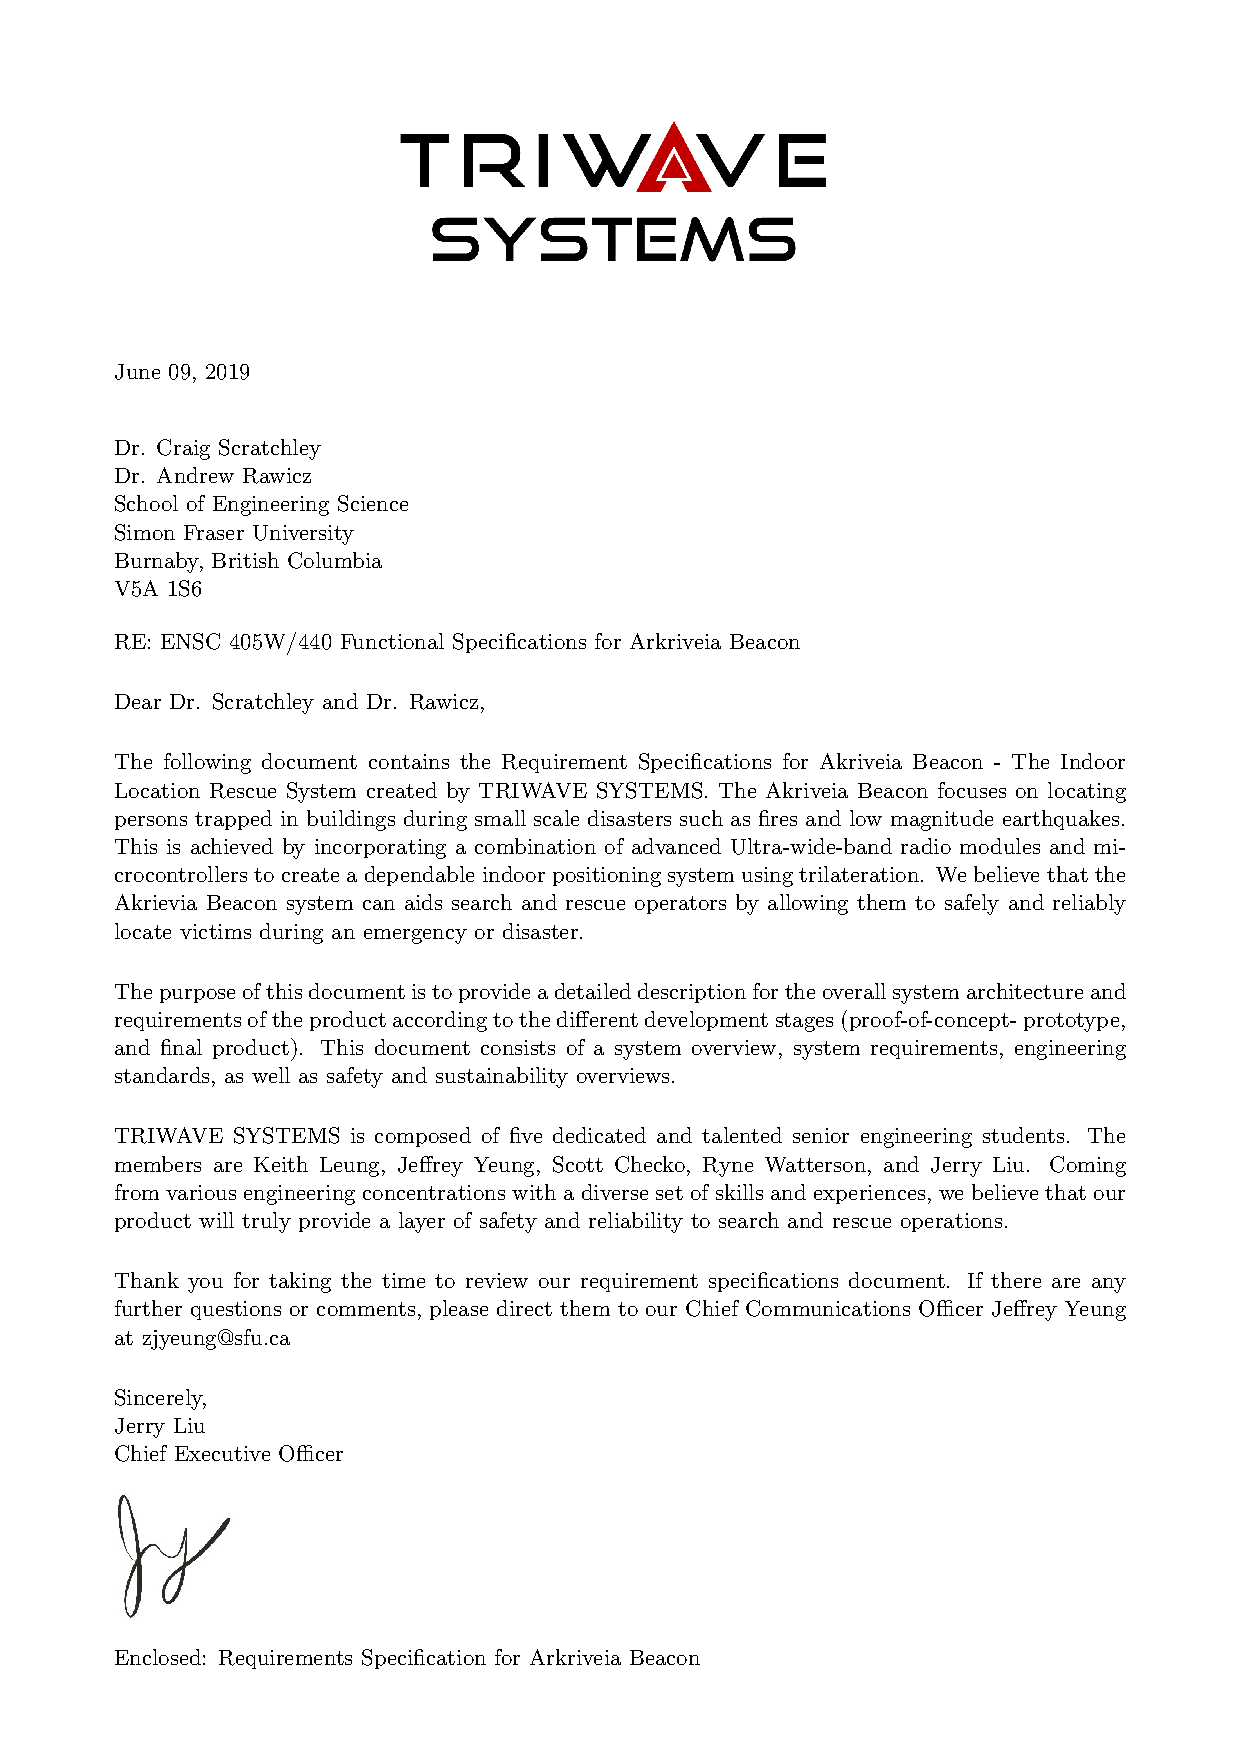
\includepdf[pages={1}]{./images/_Letter_of_transmittal.pdf}

\setboolean{@twoside}{false}

\includepdf[pages={1}]{./images/title_page.pdf}

\bigskip
%\documentclass[11pt]{article}
%\usepackage[document]{ragged2e}
%\usepackage[a4paper, total={6in, 9in}]{geometry}
%\usepackage{graphicx}
%\usepackage{float}
%\usepackage{multirow}
%\usepackage{array}
%\begin{document}


\begin{abstract}
\medskip
The Akriveia Beacon by TRIWAVE SYSTEMS focuses on improving the locating and rescue process of personnels trapped in buildings during or after small scale disasters such as fires and low magnitude earthquakes. This is achieved by incorporating an combination of advanced Ultra-wide-band radio modules, microcontroller units and data processing server to create an dependable indoor positioning system using reliable trilateration techniques. Akriveia Beacon allows search and rescue operations to safely and reliably locate victims during and after an emergency or disaster. By pinpointing the exact location of any victim wearing an ID tag, this allows rescue operators minimizing the search and rescue time; which is crucial during the time period right after a disaster strikes.

\bigskip
This document addresses the functional and nonfunctional requirements for Akriveia Beacon - The Indoor Location Rescue System created by TRIWAVE SYSTEMS. From this document, the reader will be able to gain full understanding to the functions and higher-level system design of the Akriveia Beacon. The specifications details system components, and requirements for each specified domains. Additionally aspects of engineering standards, responsibilities, safety, and sustainability of this project are outlined to provide an overview for practices followed by the engineers at TRIWAVE SYSTEMS.

\bigskip
TRIWAVE SYSTEMS is dedicated to creating a reliable and robust system for disaster search and rescue operations with human safety as the pivotal focus.

\end{abstract}
%\end{document}

\pagebreak
\clearpage
\printglossaries
\pagebreak
\begin{spacing}{0.85}
\tableofcontents
\end{spacing}
\pagebreak
\listoffigures
\pagebreak
\listoftables
\pagebreak


\setcounter{section}{0}
\section{Introduction}
\bigskip

\subsection{Background}
Over the last couple of decades urban centers around the world have faced substantial population growth. As a result, the number of large and complex structures in dense urban areas around the world is rapidly increasing. In Canada alone there are approximating 500,000 commercial buildings \cite{R1}. A large population combined with massively complex buildings in relatively dense areas leads to higher risk for damage and casualties in the event of a disaster. Due to increased urbanization and complexity of urban structures, search and rescue operations in indoor urban environments face various complications and uncertainties. According to Statistics Canada, an average of 135 fire related deaths occur with commercial structures each year from 2010 to 2014 \cite{R2}.

\bigskip
In current practices, first responders know little about the situation until arriving on scene. Once responders are on scene, emergency management have to quickly evaluate the situation and take appropriate actions \cite{R3}.  Assessments of the structure are conducted with readily available blueprints of buildings along with limited information of last known location of possible trapped victims, usually derived from witness reports. Situational data are created dynamically during this process and the actual rescue process heavily depends on the situational awareness of the first line of emergency response operators \cite{R4}.

\bigskip
An important issue that must be considered is how emergency first responders should be dispatched inside the building in the event of a disaster in order to minimize search and rescue time. In order to pinpoint locations of trapped victims quickly and accurately it is critical to have precise data. Proper emergency planning and organization takes a substantial amount of time, and having additional accurate information on the locations of trapped, incapacitated or immobile personnel would improve first responders situational awareness which would then improve their own safety and possibly greatly increases the victims chances of rescue and survival.

\bigskip
As such, the need for a distinct indoor positioning rescue system is crucial in getting fast and reliable information that allows first responders to be dispatched within the builds in the most optimal and efficient manner. The Akriveia Beacon by TRIWAVE SYSTEMS focuses on improving the locating and rescue process of personnel trapped in buildings during or after small scale disasters such as fires and low magnitude earthquakes. This is done through a system of Ultra Wide-Band (\Gls{UWB}) Beacons and \Gls{ID} tags for accurate, near real-time location of trapped personnel.

\bigskip
Ultra-Wideband radio modules are small radio transceivers using ultra-wide band radio spectrum to communicate with one another. Each ID tag uses a UWB transceiver module to communicate with the beacon system with similar UWB transceivers. Given the time between sending and receiving transmission data, the distance can be estimated via \Gls{RSSI} or time of flight. The Beacons will then forward these distance estimations to a data processing unit using a closed Wi-fi network where it will use trilateration to calculate the near real time location of each individual ID tag. The system design allows for multiple ID tags as well as more than three anchor beacons to provide more accuracy through redundancy, making it modular and extendible.

\break
\subsection{Scope}
\medskip
The Akriveia Beacon product is developed through three different phases of development as shown in Figure \ref{dev}. The three different phases including: the proof-of-concept phase, prototype phase, and final product phase. A high-level design of the system hardware and software is presented in this document to demonstrate the overall system architecture, functionality and implementation of the Akriveia beacon product. The design section of this document is divided into four main sections, overall system design, hardware design, electrical design, and software design. These design specification will indicate the components, implementations, requirements, and constraints that must be met and satisfied within the project time frame. 

\medskip
\begin{figure}[H]
\centering
    
\includegraphics[scale=0.5]{./images/dev-path.png}
    \caption{Development Cycle}
    \label{dev}
\end{figure}


\subsection{Intended Audience}
\medskip
This document is presented by engineers at TRIWAVE SYSTEMS as a guide for the design and system overview of the Akriveia Beacon product. The intended audience of this document includes but not limited to, potential clients and/or partners, the supervising professors Dr. Craig Scratchley and Dr. Andrew Rawicz, associated teaching assistants and fellow TRIWAVE SYSTEMS members. The hardware and software engineers of the project can reference this document during the various stages of development and testing stages of the project for clarification. Near the completion of the prototype development phase the product will be tested against the cases specified in the test plan. Engineers responsible for performing quality assurance can refer to the Appendix of this document to ensure all safety concerns have been addressed and that the product fulfils all requirements and meets all expectations for proper usage. 

\break
\subsection{Design  Classification}
For consistency purposes, the following design classification code convention is used to describe and organize design requirements listed throughout this document. 
\medskip
\begin{center}
	\textbf{[ DES.SE.\# - X ]} 
\end{center}

\bgroup
\def\arraystretch{1.5}
\begin{table}[H]
\centering
\begin{tabular}{ | m{1cm} | m{13cm}| } 
\hline
\rowcolor{lightgray} \textbf{Code} & \textbf{Definition} \\ 
\hline
 \textbf{DES} & Design abbreviation. \\ 
\hline
 \textbf{SE} & Design Domain Abbreviation Code correspond with each Design requirements. (see Table 2)\\   
\hline
 \textbf{\#} & Design number ID \\ 
\hline
 \textbf{X} & Development Stage Encoding (see Table 3)\\ 
\hline
\end{tabular}
\caption{Design Requirement Encoding}
\end{table}

\bgroup
\def\arraystretch{1.5}
\begin{table}[H]
\centering
\begin{tabular}{ | m{7cm} | m{7cm}| } 
\hline
\rowcolor{lightgray} \textbf{Requirement Domain} & \textbf{Abbreviation Code} \\ 
\hline
 System & SY\\ 
\hline
 Hardware & HW\\ 
\hline
 Electrical & EC\\  
\hline
 Software & SW\\ 
\hline
\end{tabular}
\caption{Design  Domain Abbreviation Code}
\end{table}

\bgroup
\def\arraystretch{1.5}
\begin{table}[H]
\centering
\begin{tabular}{ | m{7cm} | m{7cm}| }
\hline
\rowcolor{lightgray} \textbf{Development Stage} & \textbf{Encoding} \\
\hline
Proof of Concept & C\\
\hline
Prototype & P\\
\hline
Final Product & F\\
\hline
\end{tabular}
\caption{Development Stage Encoding}
\end{table}	













\pagebreak


\setcounter{section}{1}
\section{System Overview}
\bigskip

The Akriveia Beacon indoor locating rescue system combines hardware, electrical, and software systems to detect and locate multiple occupants within a building during an emergency disaster situation. Each individual component of the system is developed separately in the PoC (Proof of Concept) phase; then partially integrated in the Prototype phase and fully integrated in the Final Product phase. 

\bigskip
A high-level system overview presents three Locator Beacons, an ID tag, a data processing unit, and a graphical user interface (Figure \ref{sys_arch}). Using ultra-wideband (3.5-6.5 GHz) wireless communication the Locator Beacons transmit signals to the ID tag to acquire a response. When the response returns back to the Beacon a time of flight measurement is acquired. The Time-of-Flight principle (ToF) is a method for measuring the distance between a sensor and an object, based on the time difference between the emission of a signal and its return to the sensor, after being reflected by an object. \cite{R2-0}. The ToF data will be forwarded to the portable data processing unit via a closed Wi-Fi network with UDP.  Then the processing unit will calculate the distance and coordinates of the ID tags using trilateration algorithm. Afterwards, the coordinates results are displayed on a GUI for operators.

\medskip
\begin{figure}[H]
\centering
    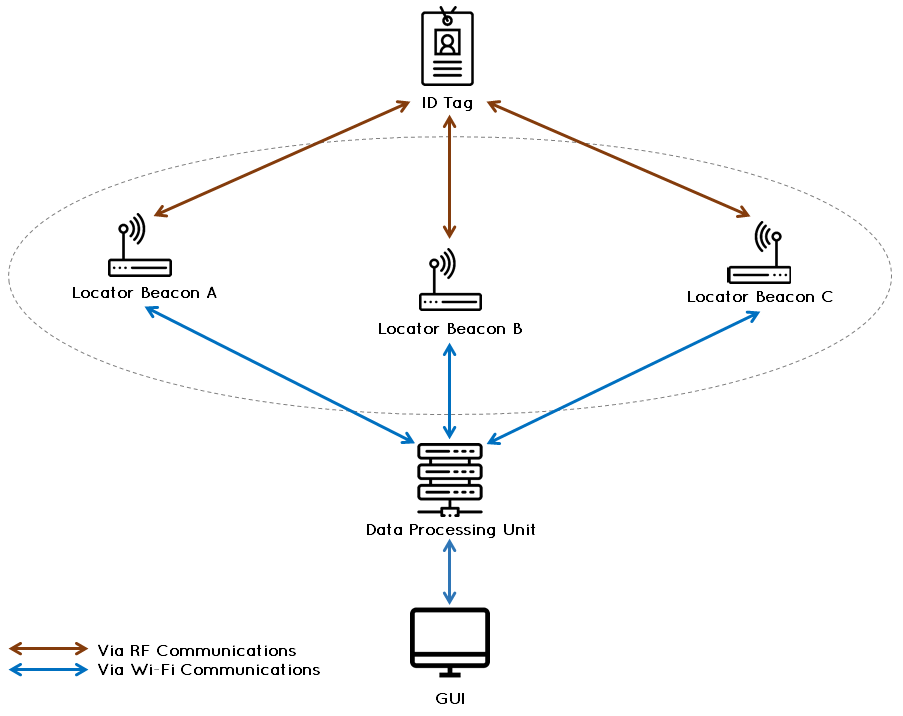
\includegraphics[scale=0.65]{./images/00_sys_arch.png}
    \caption{High Level System Layout}
    \label{sys_arch}
\end{figure}



\pagebreak
\subsection{Proof of Concept}
\medskip
The Proof of concept phase demonstrates the feasibility and functionality of an indoor location determination system. The PoC system will evaluate how effect a trilateration method is to determine the distance and location of a mobile  ID tag in two dimensional space as well as to establish an initial development system. Similar to the system block diagram shown in figure \ref{poc}.

\bigskip
ESP32 micro-controllers are used as the main hardware components of the Beacon and ID Tags. The ESP32 is an off the shelf, low-cost, low-power system on a chip micro-controllers with integrated Wi-Fi and dual-mode Bluetooth. Received Signal Strength Indicator (RSSI) from Bluetooth Low Energy (BLE) modules are used to estimate distance between each beacon and ID tag. Each beacon determines the MAC address and a RSSI measurement from the advertising ID Tag. The data is forwarded to the data processing unit - Raspberry Pi, via USB serial communication. The RSSI is then used to estimate distance between each ID Tag and the associating Beacon and the results are output to a simple UI. 

\medskip
\begin{figure}[H]
\centering
    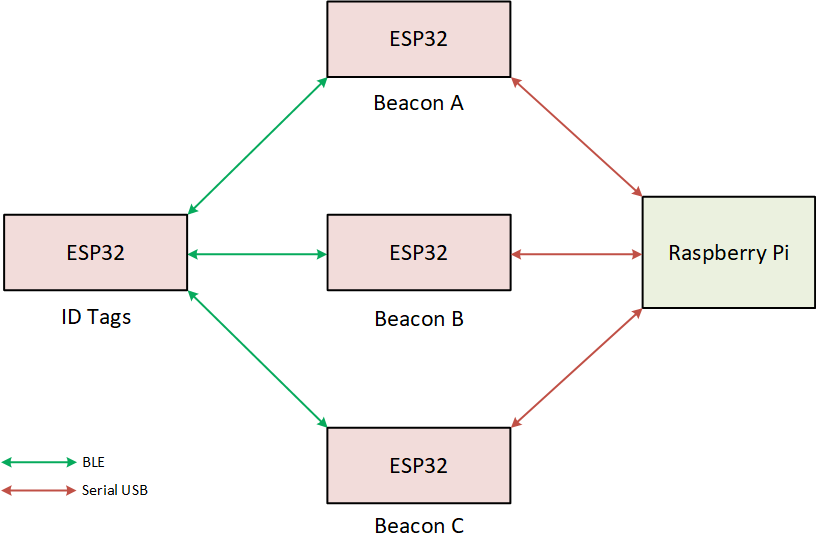
\includegraphics[width=\linewidth]{./images/01_poc.png}
    \caption{PoC System Block Diagram}
    \label{poc}
\end{figure}



\pagebreak
\subsection{Prototype}
\medskip
In the Prototype development phase the transceivers will be incorporated with Decawave DWM1000 UWB modules. The DWM1000 UWB uses radio frequencies in the range of 3.5 to 6.5 GHz; this would significantly reduce issues of signal interference or multipath propagation which would occur by using RSSI with BLE. The DWM1000 will be incorporated as the transceiver with the ESP32 as the main MCU as shown in figure \ref{prototype} below. RF data communication functions will be established between four UWB modules with one as the ID Tag and three as the Locator Beacons to demonstrate distance estimation with DWM1000 UWB modules. This will be achieved by using signal fingerprinting to determine transmitter properties such as ToF and unique Tag identifier. Furthermore, trilateration algorithms will be implemented on data processing unit to determine near real time location and coordinates of ID Tags. Initial Implementation of software stack on data processing unit and development of GUI will occur during this phase as well.

\medskip
\begin{figure}[H]
\centering
    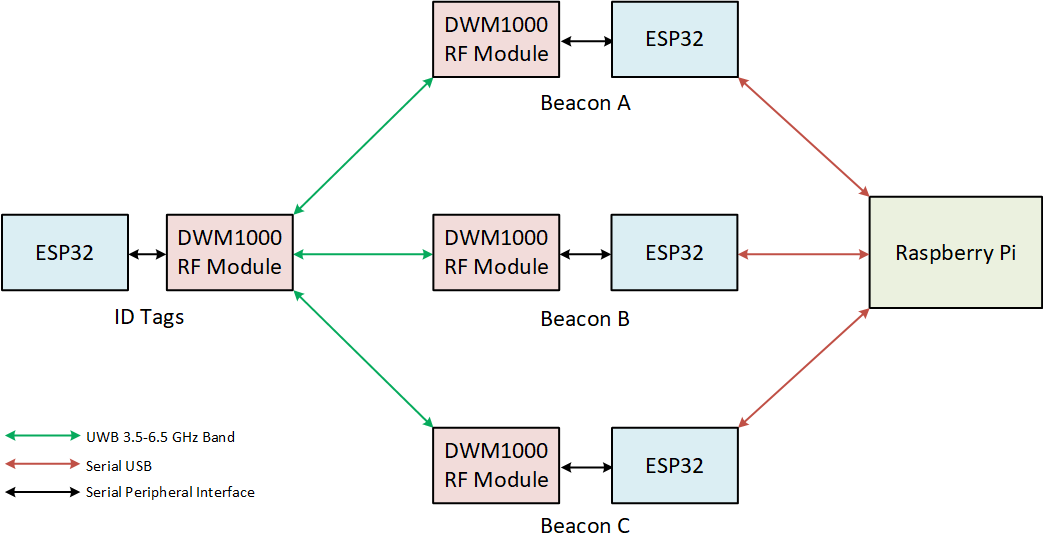
\includegraphics[width=\linewidth]{./images/02_prototype.png}
    \caption{Prototype System Block Diagram}
    \label{prototype}
\end{figure}


\pagebreak
\subsection{Final Product}
\medskip
The final product will demonstrate the fully functional indoor rescue system that detects the location of the ID tags and displays it accordingly on a GUI. Here the addition of ESP32’s Wi-Fi modules can be seen (Figure \ref{final}), as the Beacon will communicate via Wi-Fi communication with the data processing unit. The Wi-Fi network will be a closed network meaning that the network is only share between beacons and the data processing unit to ensure security, reliability and stability. Furthermore, implementation of RF harvesting circuit for ID Tag device charging during deep sleep mode will occur during this stage. All the components of the systems will be fully integrated as a close-to-production product. Component circuits and PCB footprint will be minimized and proper casing will be made to house all electronics. The data processing unit will provide the user with a full GUI to interact with the system along with the fully implemented features such as importable blueprints and multi-floor tracking.

\medskip
\begin{figure}[H]
\centering
    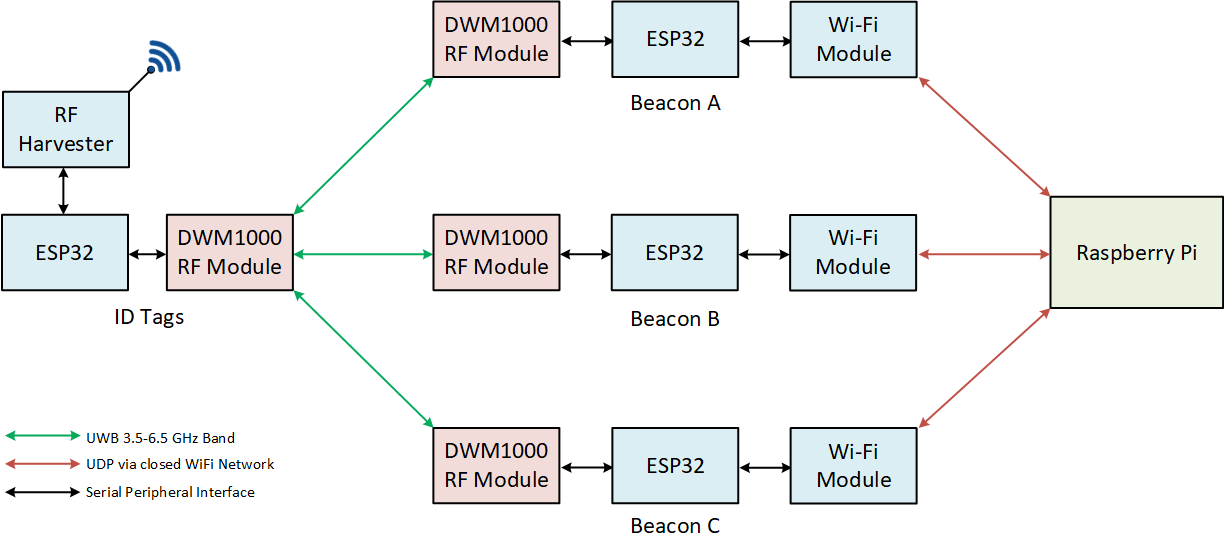
\includegraphics[width=\linewidth]{./images/03_final.png}
    \caption{Final System Block Diagram}
    \label{final}
\end{figure}




\pagebreak
\subsection{Ultra-Wideband Radio Technology}
\medskip



\pagebreak
\subsection{Trilateration Methods}



\pagebreak
%\documentclass[11pt]{article}
%\usepackage[a4paper, total={6.5in, 9.5in}]{geometry}
%\usepackage[document]{ragged2e}
%\usepackage{lipsum}
%\usepackage{graphicx}
%\usepackage{float}
%\usepackage{multirow}
%\usepackage{array}
%\usepackage{cellspace}
%\usepackage{etoolbox}
%\usepackage{scrpage2}
%\usepackage{longtable}
%\usepackage[table, svgnames]{xcolor} 
%\ifoot[]{}
%\cfoot[]{}
%\ofoot[\pagemark]{\pagemark}
%\pagestyle{scrplain}
%
%\begin{document}

\setcounter{section}{2}
\section{System Requirements}
\bigskip
TRIWAVE SYSTEMS is dedicated on producing a high-quality product. To ensure production quality, various requirements at different stages of development will be stated clearing in this section. These requirements will be covering from all aspects of the Akriveia Beacon technology. TRIWAVE SYSTEMS has decided that the following requirements, when met, will ensure that this product will be an asset to all first responders that use it, in as many emergency situations as possible. As TRIWAVE SYSTEMS puts a high price on safety, reliability, and ease of use, so that this product may help save lives and keep first responders safe.  The functionalities that are labelled with a '\textbf{C}', as Proof-of-Concept, will be presented at the end of ENSC 405W.

\bigskip
\textit{Note: Requirements marked with ‘*’ are not carried over into subsequent development phases}


\bigskip
\subsection{General Requirements}
In order for the Akriveia Beacon system to be reliable, general high-level requirements describing the important core functions of the system are detailed in the table below. By following these requirements, TRIWAVE SYSTEMS ensure the overall system function and intended purpose are met at every phase of the development cycle.

\bigskip

\bgroup
\def\arraystretch{1.5}
\begin{table}[H]
\centering
\begin{tabular}{ | m{3.25cm} | m{12.5cm} |} 
 \hline
 \textbf{REQ.GE.1 - C} & The system must be intended for indoor use only \\ 
\hline
 \textbf{REQ.GE.3 - C} & The system must have two modes of operation: idle mode and emergency mode \\ 
\hline
 \textbf{REQ.GE.4 - C} & The system must pinpoint ID tag location within one floor buildings \\
\hline
 \textbf{REQ.GE.5 - C} & Access to the system and system data must not be available to the general public \\
\hline
 \textbf{REQ.GE.6 - P} & First responders must only have access to the system during disaster situation \\
\hline
 \textbf{REQ.GE.7 - P} & The system must track more than one ID tag \\
\hline
 \textbf{REQ.GE.8 - F} & The system must locate ID tags in a building with multiple floors \\
\hline
 \textbf{REQ.GE.9 - F} & The system must remain operational after earthquakes with magnitude below 6.9 \\
\hline
 \textbf{REQ.GE.10 - F} & The system must remain operational after or during small scale fires \\
\hline
 \textbf{REQ.GE.11 - F} & The final marketed product must not cost more than CAD \$200.00 \\
\hline
\end{tabular}
\caption{General Requirements}
\end{table}	

\break
\subsection{Hardware Requirements}
Robust and reliable hardware will be absolutely necessary in any system that interacts with emergency disaster management. TRIWAVE SYSTEMS has chosen to develop the proof-of-concept prototype using 2.4 GHz radio modules as feasibility testing, before upgrading the system to using Ultra Wide Band (UWB) modules for further prototyping. Micro-controller Units (MCUs) will be used to control the beacons and ID tags. The requirements below details the requirement for hardware functionality of the Akrivia Beacon system.

\bigskip

\bgroup
\def\arraystretch{1.5}
\begin{table}[H]
\centering
\begin{tabular}{ | m{3.25cm} | m{12.5cm} |} 
 \hline
 \textbf{REQ.HW.1 - C} & The server must use a SBC for automated product control \\ 
\hline
 \textbf{REQ.HW.2 - C} & The beacons must use a MCU for automated product control \\ 
\hline
 \textbf{REQ.HW.3 - C} & The ID tags must use a MCU for automated product control \\ 
\hline
 \textbf{REQ.HW.4 - C} & Each MCU must use Serial Peripheral Interface (SPI) to communicate with transceiver \\
\hline
 \textbf{REQ.HW.5 - C*} & The beacons must use 2.4 GHz radio modules as transceivers* \\
\hline
 \textbf{REQ.HW.6 - C*} & The ID tags must use 2.4 GHz radio modules as transceivers*  \\
\hline
 \textbf{REQ.HW.7 - C*} & The beacons must communicate with the server via serial USB* \\
\hline
 \textbf{REQ.HW.8 - P} & The beacons must communicate with the server via either RS485 or Ethernet  \\
\hline
 \textbf{REQ.HW.9 - P} & The beacons must use 3.5-6.5 GHz UWB radio modules as transceivers \\
\hline
 \textbf{REQ.HW.10 - P} & The ID tags must use 3.5-6.5 GHz UWB radio modules as transceivers \\
\hline
\end{tabular}
\caption{Hardware Requirements}
\end{table}	

\break
\subsection{Electrical Requirements}
Since the system is designed for emergency disaster situations, it is crucial that sufficient power is provided to each device at any given time. In order for the system to be reliable and effective, the electrical systems must be robust and efficient. TRIWAVE SYSTEMS has compiled a strict set of electrical requirements that ensures the beacons and ID tags will operate at a safe and efficient state. 

\bigskip

\bgroup
\def\arraystretch{1.5}
\begin{table}[H]
\centering
\begin{tabular}{ | m{3.25cm} | m{12.5cm} |} 
 \hline
 \textbf{REQ.EC.1 - C} & Each beacon shall be powered through standard North American power outlets (120V AC, 60Hz, type A/B) \\ 
\hline
 \textbf{REQ.EC.2 - C} & Each ID tag must have its own 3.3 V battery power source \\ 
\hline
 \textbf{REQ.EC.3 - P} & Each ID tag must have an on-off toggle switch  \\ 
\hline
 \textbf{REQ.EC.4 - P} &  Each ID tag must remain in an idle, low power state with no more than 5W of power consumption while not in a disaster  \\
\hline
 \textbf{REQ.EC.5 - P} &  Each beacon must remain in an idle, low power state with no more than 5W of power consumption while not in a disaster \\
\hline
 \textbf{REQ.EC.6 - P} & Each beacon shall have its own backup power source (9V battery)  \\
\hline
 \textbf{REQ.EC.7 - P} & Each ID tag will use RF power harvesting technology to maintain charge on its batteries \\
\hline
 \textbf{REQ.EC.8 - F} &  Each ID tag must have a primary switch using an additional RF harvester as the trigger and a secondary manual switch to turn device on only   \\
\hline
 \textbf{REQ.EC.9 - F} & Each beacon shall incorporate a power caster device \\
\hline
 \textbf{REQ.EC.10 - F} & The server must have a battery backup (UPS) \\
\hline
\end{tabular}
\caption{Electrical Requirements}
\end{table}	

\break
\subsection{Software Requirements}
The Akriveia system will composed a intricate software stack containing a database and a web server hosted GUI. The server is the main data processing using and will be implemented with trilateration algorithms to locate ID tag positions in near real time. In order for the software system to be reliable, secure and accurate the following requirements were made.

\bigskip

\bgroup
\def\arraystretch{1.5}
\begin{longtable}[H]{ | m{3.5cm} | m{12.5cm} |} 
 \hline
 \textbf{REQ.SW.1 - C} & The system must use time of flight to locate ID tags \\ 
\hline
 \textbf{REQ.SW.2 - P*} & The system must use 2D trilateration methods to locate ID tags* \\ 
\hline
 \textbf{REQ.SW.3 - P} & Distance calculations must be performed using RSSI data received from beacons \\ 
\hline
 \textbf{REQ.SW.4 - P} & Admin shall have access the the server through credential verification system \\
\hline
 \textbf{REQ.SW.5 - P} & Admins must be able to create employees account associated with each ID tag \\
\hline
 \textbf{REQ.SW.6 - P} & First responder ID tags must be assicated with pre-define first responder account \\
\hline
 \textbf{REQ.SW.7 - P} & The server must be able to periodically check ID tags to verify tags are in working condition (correctness of data, device not broken) \\
\hline
 \textbf{REQ.SW.8 - P} & The system must detect and report ID tag defects, if any \\
\hline
 \textbf{REQ.SW.9 - P} & The server will store location history through out the event of an emergency \\
\hline
 \textbf{REQ.SW.10 - F} & Scaled blueprints of the monitor area must be able to be uploaded to the server system for accurate layout and location \\
\hline
 \textbf{REQ.SW.11 - F} & The ID tags broadcasting must be able to be turned off from the servers \\
\hline
 \textbf{REQ.SW.12 - F} & The server must distinguish between different floors and be able to provide locations of ID tags for any floor serviced at any time during an emergency \\
\hline
 \textbf{REQ.SW.13 - F} & The system will provide floor plans for operators to track locations of disaster victims \\
\hline
 \textbf{REQ.SW.14 - F} & The system must use 3D trilateration methods to locate ID tags \\
\hline
\caption{Software Requirements}
\end{longtable}	

\break
\subsubsection{Software - UI Requirements}
Emergency first responders will be the first operators to interact with the Akriveia beacon system during a disaster. As such, the user interface must be intuitive and quick to use for the first responders. The following table highlight important user interface requirements of the system.
\bigskip

\bgroup
\def\arraystretch{1.5}
\begin{longtable}[H]{ | m{3.5cm} | m{12.5cm} |} 
\hline
 \textbf{REQ.SW.15 - P} & The \Gls{UI} must be intuitive to use for operators \\
\hline
 \textbf{REQ.SW.16 - P*} & The system must display a simple floor-plan/blueprint represented as simple geometry (ie. rectangle)* \\
\hline
 \textbf{REQ.SW.17 - P} & The system UI must display location of ID tags in near real time \\
\hline
 \textbf{REQ.SW.18 - P} & Each ID tags must be identified on the UI map by distinct symbols and/or tags \\
\hline
 \textbf{REQ.SW.19 - P} & The system UI application must fill the entire screen but not obscure any system-wide status bars. \\
\hline
 \textbf{REQ.SW.20 - P} & UI tag for rescue operations must have distinct indication from civilian ID tags \\
\hline
 \textbf{REQ.SW.21 - F} & The System UI must support mobile devices such as laptop PCs and \Gls{iOS} tablets \\
\hline
 \textbf{REQ.SW.22 - F} & The UI must be able to display blueprints and location markers for all serviced floors in building \\
\hline
\caption{Software - UI Requirements}
\end{longtable}	
\break

\subsection{Performance Requirements}
Reliability and accuracy are the most important attributes of the Akriveia system during an emergency situation. As a system designed to be widely used by first responders, the Akriveia Beacons must be both reliable and accurate. Performance of the product maintain top priority before the system reach general availability. The requirements below reflect the importance TRIWAVE SYSTEMS puts on the performance of the Akriveia Beacon system.

\bigskip
\bgroup
\def\arraystretch{1.5}
\begin{table}[H]
\centering
\begin{tabular}{ | m{3.5cm} | m{12.5cm} |} 
 \hline
 \textbf{REQ.PE.1 - C*} & The system shall locate users within the building with an accuracy of 1m* \\ 
\hline
 \textbf{REQ.PE.2 - P} & The system shall track each ID tag in near real time with a latency of no more than 3 seconds \\ 
\hline
 \textbf{REQ.PE.3 - P} & The system must undergo a calibration process on start-up before usage \\ 
\hline
 \textbf{REQ.PE.4 - P} & The system UI must be accessible with in 60 seconds when operators directly connect to the system server \\
\hline
 \textbf{REQ.PE.5 - F} & The system shall locate users within the building with an accuracy of 0.5m \\
\hline
 \textbf{REQ.PE.6 - F} & The server's location processing throughput must be at least 100 employee locations per second \\
\hline
 \textbf{REQ.PE.7 - F} & Each beacon must be capable of detecting at least 100 employees within a 100m radius in 1 second \\
\hline
 \textbf{REQ.PE.8 - F} & The ID Tags must remain operational under temperatures no more than 60 degree Celsius \\
\hline
 \textbf{REQ.PE.9 - F} & The Beacons must remain operational under temperatures no more than 60 degree  \\
\hline
\end{tabular}
\caption{Performance Requirements}
\end{table}	

\break

\subsubsection{Performance Requirements - Signal}
In addition to basic performance requirement, the Akriveia beacon heavily relies on wireless signal communications. The following tables details the requirements for signal communication and processing.
\bigskip

\bgroup
\def\arraystretch{1.5}
\begin{table}[H]
\centering
\begin{tabular}{ | m{3.5cm} | m{12.5cm} |} 
\hline
 \textbf{REQ.PE.10 - C*} & 50\% of data transmitted via wireless communication must not be lost or corrupted* \\
\hline
 \textbf{REQ.PE.10 - C*} & Wireless communication must be done using 2.4 GHz wireless frequencies* \\
\hline
 \textbf{REQ.PE.10 - C*} & Wireless communication between transceivers must not have a latency of more than 100ms* \\
\hline
 \textbf{REQ.PE.10 - P} & The latency of wireless communication between transceivers must be less than 50ms \\
\hline
 \textbf{REQ.PE.10 - P} & Wireless communication must be established on 3.5-6.5 GHz UWB frequencies \\
\hline
 \textbf{REQ.PE.10 - F} & 5\% of data transmitted via wireless communication must not be lost or corrupted \\

\hline
\end{tabular}
\caption{Performance - Signal Requirements }
\end{table}	
	
%\end{document}
\pagebreak
%\documentclass[11pt]{article}
%\usepackage[document]{ragged2e}
%\usepackage[a4paper, total={6.5in, 9.5in}]{geometry}
%\usepackage{graphicx}
%\usepackage{float}
%\usepackage{multirow}
%\usepackage[table, svgnames]{xcolor} 
%\usepackage{array}
%\usepackage{cellspace}
%\usepackage{etoolbox}
%\begin{document}

\setcounter{section}{3}
\section{Engineering Standards \& Responsibilities}
\bigskip
The Akriveia Beacon will be designed to meet various engineering standards published by the IEEE, the IEC, the ISO, and the CSA Group to ensure performance and safety of the final product. The system contain electronics, software, and communication protocols, which means that suitable standards must be followed. The data communication on physical layer is done using frequency on the ultra-wideband spectrum operating in unlicensed frequency bands, wireless standards that apply to the operation band will be followed. Akriveia Beacon is designed to operate during disaster situations, material and design must follow the structural and durability standards for disaster equipments. 


\subsection{Electronics Standards}
\bgroup
\def\arraystretch{1.5}
\begin{table}[H]
\centering
\begin{tabular}{ |p{3cm} p{11cm} | }
\hline
\multicolumn{1}{|r|}{IEEE 1625} & IEEE Standard for Rechargeable Batteries for Multi-Cell Mobile Computing Devices []\\ 
\hline
\multicolumn{1}{|r|}{CSA-C22.2 NO.61508-1:17} & Functional safety of electrical/electronic/programmable electronic safety-related systems - Part 1: General requirements []\\ 
\hline
\multicolumn{1}{|r|}{CSA-C22.2 NO.0.23-15} & General requirements for battery-powered appliances []\\  
\hline
\multicolumn{1}{|r|}{CAN/CSA-C22.2 NO.0-10} & General requirements - Canadian electrical code, part II []\\ 
\hline
\multicolumn{1}{|r|}{IEEE P360} & Standard for Wearable Consumer Electronic Devices - Overview and Architecture [] \\  
\hline
\end{tabular}
\caption{Electronics Standards}
\end{table}	
\medskip


\subsection{Wireless Standards}
\bgroup
\def\arraystretch{1.5}
\begin{table}[H]
\centering
\begin{tabular}{ | p{3.5cm} | p{11.5cm}| } 
\hline
\multicolumn{1}{|r|}{IEEE 802.15.2-2003} & IEEE Recommended Practice for Information technology-- Local and metropolitan area networks-- Specific requirements-- Part 15.2: Coexistence of Wireless Personal Area Networks with Other Wireless Devices Operating in Unlicensed Frequency Bands []\\ 
\hline
\multicolumn{1}{|r|}{IEEE 802.15.4q-2016} & IEEE Standard for Low-Rate Wireless Networks --Amendment 2: Ultra-Low Power Physical Layer []\\ 
\hline
\multicolumn{1}{|r|}{ISO/IEC 26907:2009} & Information technology -- Telecommunications and information exchange between systems -- High-rate ultra-wideband PHY and MAC standard []\\  
\hline
\multicolumn{1}{|r|}{ISO/IEC 24730-62:2013} & Information technology -- Real time locating systems (RTLS) -- Part 62: High rate pulse repetition frequency Ultra Wide Band (UWB) air interface []\\  
\hline
\multicolumn{1}{|r|}{IEEE P802.15.4z} & Standard for Low-Rate Wireless Networks Amendment: Enhanced High Rate Pulse (HRP) and Low Rate Pulse (LRP) Ultra Wide-Band (UWB) Physical Layers (PHYs) and Associated Ranging Techniques [] \\  
\hline
\end{tabular}
\caption{Wireless Standards}
\end{table}	


\pagebreak
\subsection{Software Standards}
\bgroup
\def\arraystretch{1.5}
\begin{table}[H]
\centering
\begin{tabular}{ | p{4cm} | p{12cm}| } 
\hline
\multicolumn{1}{|r|}{IEEE 12207-2017} & ISO/IEC/IEEE International Standard - Systems and software engineering -- Software life cycle processes []\\
\hline 
\multicolumn{1}{|r|}{IEEE P2510} & Standard for Establishing Quality of Data Sensor Parameters in the Internet of Things Environment []\\ 
\hline
\multicolumn{1}{|r|}{ISO 2382-9:1984} & Data processing -- Vocabulary -- Part 9: Data communication []\\
\hline 
\end{tabular}
\caption{Software Standards}
\end{table}	
\medskip

\subsection{Material Standards}
\bgroup
\def\arraystretch{1.5}
\begin{table}[H]
\centering
\begin{tabular}{ | p{4cm} | p{12cm}| }
\hline
\multicolumn{1}{|r|}{IEEE 1221-1993} & IEEE Guide for Fire Hazard Assessment of Electrical Insulating Materials in Electrical Power Systems []\\ 
\hline
\multicolumn{1}{|r|}{IEEE 848-2015} & IEEE Standard Procedure for the Determination of the Ampacity Derating Factor for Fire-Protected Cable Systems []\\ 
\hline
\end{tabular}
\caption{Material Standards}
\end{table}	


%\end{document}
\pagebreak
%\documentclass[11pt]{article}
%\usepackage[document]{ragged2e}
%\usepackage[a4paper, total={6.5in, 9.5in}]{geometry}
%\usepackage{graphicx}
%\usepackage{float}
%\usepackage{multirow}
%\usepackage[table, svgnames]{xcolor} 
%\usepackage{array}
%\usepackage{cellspace}
%\usepackage{etoolbox}
%\begin{document}

\setcounter{section}{4}
\section{Safety \& Sustainability}
\bigskip
\subsection{Safety}
\medskip
The Akriveia Beacon system is a combination of electronics, wireless communication, and software systems all functioning together to create a reliable solution. Since the system is designed for disaster related situations, safety is paramount. There are essentially two conditions the system would be under; an idle mode from day to day; and an emergency mode where the system is trigger to transmit location data during a real disaster situation.

\bigskip
During idle mode or normal day to day operations the ID tags would be worn much like an access card. As such, electronic components on the ID tags must agree to standardized safety measurements. During emergency mode under a disaster situation, the beacons are turned on to transmit and receive data from the ID tags. As the associated ID tags will be transmitting ultra-wideband radio frequency both to and from the radio modules which will be worn by a person, the power frequency level must be within limits that are safe for human exposure [safe1]. Additionally, the Akriveia Beacon system will satisfy the following safety requirements:

\bgroup
\def\arraystretch{1.5}
\begin{table}[H]
\centering
\begin{tabular}{ | m{3cm} | m{13cm}| } 
\hline
REQ & C\\ 
\hline
REQ & P\\ 
\hline
REQ & F\\  
\hline
\end{tabular}
\caption{Safety Requirements}
\end{table}	

\break
\subsection{Sustainability}
\bigskip
The engineers at TRIWAVE SYSTEMS is committed to ensuring the final products is not only functionally effective, but also in compliance with the best environmental sustainability practices. As such, TRIWAVE SYSTEMS will be dedicated to minimizing impact of the environment by making design choices that are environmentally sustainable by following the Cradle to Cradle (C2C) standards. C2C refers to the process of development where all components used in manufacturing are able to be brought back into the development cycle [sus1]. By following the C2C Certified standards, the Akriveia Beacon system can be repurposed or recycled as shown below in the figure by EPEA.

\begin{figure}[H]
\centering
    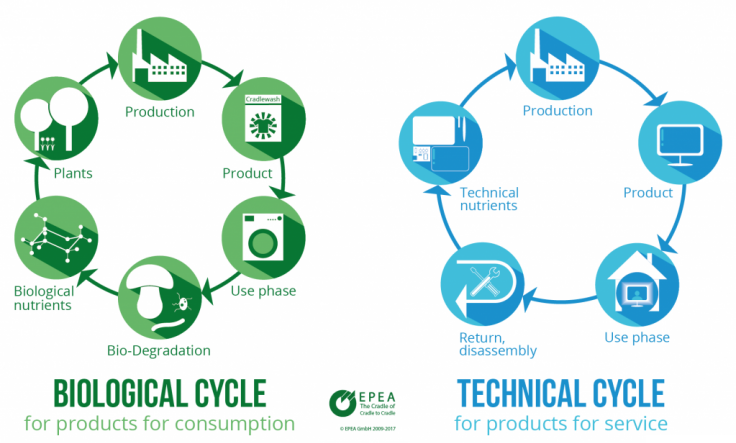
\includegraphics[scale=0.85]{./images/BioTechCycle.png}
    \caption{Biological and Technical C2C cycles [sus2]}
\end{figure}

When possible, the Akriveia Beacon will be manufactured with biodegradable and non-toxic materials, as well as materials that are easily recyclable or repurposable to ensure waste output is minimal. The material of choice for beacons and ID tag casings will be biodegradable non-toxic Polylactic acid or PLA plastics [sus3]. PLA is a natural, bio based alternative to petroleum laden ABS and used commonly in 3D printing process. Electronics and circuitry of the product will be designed with a minimal footprint. Power sustainability is also considered by incorporating the use of RF harvesting. By converting radio frequency power into DC voltage to power devices, the need for constant battery replacement is minimized lowering maintenance costs. The following table includes the sustainability requirements for the system.

\break
The following table includes the sustainability requirements for the Akriveia Beacon system:

\bgroup
\def\arraystretch{1.5}
\begin{table}[H]
\centering
\begin{tabular}{ | m{3cm} | m{13cm}| } 
\hline
REQ & C\\ 
\hline
REQ & P\\ 
\hline
REQ & F\\  
\hline
REQ & F\\ 
\hline
REQ & F\\ 
\hline
\end{tabular}
\caption{Sustainability Requirements}
\end{table}	


%\end{document}
\pagebreak


\setcounter{section}{5}
\section{Conclusion}
\bigskip
As a company TRIWAVE SYSTEMS is focused on creating the most reliable and accurate indoor location rescue system. As aforementioned, Akriveia Beacon is a system of Ultra-WideBand (UWB) radio beacons and ID tag systems communicating via UWB and using trilateration to accurately obtain near real time location of personnels within buildings during the event of a disaster. The location information which then can be reported to emergency responders and operators to provide accurate and reliable intel for the search and rescue effort. 

\bigskip
The system overview, design, and constraints of the Akriveia Beacon were clearly established. As well as to provide a detailed outline of the requirements specifications. These requirements outlines functional and non-functional requirements expected of the Akriveia Beacon product through three different phases of development including: the proof-of-concept (completed August 2019), prototype, and final product (completed December 2019).

\begin{enumerate}
\setlength\itemsep{0.25em}
	\item General requirement 
	\item Hardware requirement 
	\item Electrical requirement 
	\item Software requirement 
	\item Performance Requirements
	\item Safety requirement 
	\item Sustainability  requirement 
\end{enumerate}


Since the Akriveia Beacon product is aimed to operate in emergency disaster scenarios, various engineering standards, safety requirement must be followed to ensure usability, durability and acceptability in the market. By following the Cradle to Cradle development cycle, the product is ensured to be both innovating and environmentally sustainable. Lastly, to ensure optimal product quality control a brief Alpha stage est plan is included in the appendix at the end of this document. It details the testing procedure for the proof of concept prototype on various parts of the Akriveia Beacon system.

\bigskip
While going through the three phases of development, this document will provide a reliable
reference to ensure requirement are satisfied at each milestone, as well as to provide a strict criteria in which to compare with the final product.

%\end{document}
\pagebreak
\setcounter{section}{6}
\section{References}
\bigskip
\pagebreak
%\documentclass[11pt]{article}
%\usepackage[a4paper, total={6.5in, 9.5in}]{geometry}
%\usepackage[document]{ragged2e}
%\usepackage{lipsum}
%\usepackage{graphicx}
%\usepackage[noadjust]{cite}  
%\usepackage{float}
%\usepackage[numbib]{tocbibind}
%\usepackage{multirow}
%\usepackage{array}
%\usepackage{setspace}
%\usepackage{cellspace}
%\usepackage{etoolbox}
%\usepackage{scrpage2}
%\usepackage{longtable}
%\usepackage[table, svgnames]{xcolor} 
%\usepackage{titlesec}
%\usepackage{amsmath}
%\setcounter{secnumdepth}{4}
%\titleformat{\paragraph}
%{\normalfont\normalsize\bfseries}{\theparagraph}{1em}{}
%\titlespacing*{\paragraph}
%{0pt}{3.25ex plus 1ex minus .2ex}{1.5ex plus .2ex}
%\ifoot[]{}
%\cfoot[]{}
%\ofoot[\pagemark]{\pagemark}
%\pagestyle{scrplain}
%\begin{document}

\setcounter{section}{7}
\section{Appendix}

\subsection{Proof Of Concept(PoC) Acceptance Test Plan}
\medskip
% What testing is there supposed to be?
The PoC Acceptance Test Plan includes all the testing procedures for verifying and validating the requirement specifications under a formal test environment. The goal of the PoC Acceptance Test Plan is to ensure the basic requirements stated in the \textbf{\textit{System Requirements}} section of the document are met.

\medskip
Three main goals for the PoC testing are as follows:

\begin{enumerate} 
    \item 2.4 GHz chips are able to receive and transmit data accurately
    \item Arduino micro-controllers(MCU) receives the transmission data 
    \item Raspberry Pi receives data serially from Arduino MCU
\end{enumerate}

%The acceptance test plan will consists of the test below:
%\begin{enumerate}
%    \item System(General) Tests
%    \item Hardware Tests
%    \item Electrical Tests
%    \item Software Tests
%    \item Software - UI Tests
%    \item Performance Tests
%    \item Performance - Signal Tests
%\end{enumerate}
% Acceptance Test Plan is Long

\subsubsection{Systems (General Testing)}

\begin{table}[h!]
    \centering
    
    \begin{tabular}{|m{0.15\linewidth}|m{0.02\linewidth}|m{0.3\linewidth}|m{0.45\linewidth}|} 
    \hline
    \multicolumn{4}{|l|}{System (General) Test}  \\ 
    \hline
    REQ.ID & \multicolumn{2}{l|}{Testing Criteria} & Expected Output \\ 
    \hline
    % Row of req ID, #, Testing Criteria, Expected Output
    REQ.GE.1-C                  
    & 1
    & Ensure all tests conducted are representative of conditions indoor instead of outdoor conditions or all-terrain conditions 
    & System testing and design are representative of conditions within a building. 
    System testing does not consider the all-weather conditions nor any unpredictable outdoor conditions.\\ 
    \hline

    % Row of req ID, #, Testing Criteria, Expected Output
    \multirow{2}{*}{REQ.GE.2-C} 
    & 1 
    & System is able to switch between two modes: idle and emergency modes       
    & Switching between the idle and emergency modes are to be robust and reliable. 
    There is significant differences in power consumption, signal communication and content between the two modes. \\ 
    \cline{2-4}
    & 2 
    & Idle mode and emergency modes should show different operations 
    & MCU serial output should show different data transfer when system is in the different modes \\ 
    \hline

    % Row of req ID, #, Testing Criteria, Expected Output   
    \multirow{2}{*}{REQ.GE.3-C} 
    & 1 
    & System should determine the location of the ID tag on one floor of a building     
    & Software algorithms determine the relative location of the ID tag to the beacons. 
    Clear distances are measured between the beacons themselves or to the ID tag.~\\ 
    \cline{2-4}
    & 2 
    & System to show relative location of the ID tag     
    & A relative location of the ID tag to the approximate floor space is calculated \\
    \hline
    \end{tabular}
    \caption{PoC System(General) Requirement Test Plans}
\end{table}

\break
\subsubsection{Hardware Test Plan}

\begin{table}[h!]
    \centering
    \begin{tabular}{|m{0.15\linewidth}|m{0.02\linewidth}|m{0.3\linewidth}|m{0.45\linewidth}|} 
    \hline
    \multicolumn{4}{|l|}{Hardware Tests}           \\ 
    % -----DONT NEED TO CHANGE THIS SECTION -----
    \hline
    REQ.ID & \multicolumn{2}{l|}{Testing Criteria} & Expected Output         \\ 
    \hline
    % ----DONT NEED  TO CHANGE THIS SECTION ----
    % Row of req ID, #, Testing Criteria, Expected Output
    REQ.HW.1-C                  
    & 1 
    & Data processing unit should use SBC to be the automated product control
    & SBC should take all received data and perform calculations   \\ 
    \hline
   
    % Row of req ID, #, Testing Criteria, Expected Output
    REQ.HW.2-C                  
    & 1 
    & Beacons to use the MCU to be the automated product control
    & MCU should control signal transmission through the 2.4 GHz chips and be fully operational 
    when used as the automated product control         \\ 
    \hline
    
    % Row of req ID, #, Testing Criteria, Expected Output
    \multirow{2}{*}{REQ.HW.3-C} 
    & 1 
    & ID tags to use the MCU to be the automated product control
    & MCU should control signal transmission through the 2.4 GHz chips and be fully operational 
    when used as the automated product control            \\ 
    \cline{2-4}
    & 2 
    & MCU should receive signals from the beacons and transmit signal back through MCU  
    & Arduino serial output for ID tag should show data received and send proper data output        \\
    \hline
    
    % Row of req ID, #, Testing Criteria, Expected Output
    REQ.HW.4-C                  
    & 1 
    & SPI should be used as the interface with the MCU and transceiver
    & Arduino serial output for MCU should show proper data transfer through the 2.4 GHz transceiver   \\ 
    \hline
    
    % Row of req ID, #, Testing Criteria, Expected Output
    \multirow{2}{*}{REQ.HW.5-C} 
    & 1 
    & Beacons should use 2.4 GHz radio frequency as the receiver     
    & Correct data input received from the 2.4 GHz radio module          \\ 
    \cline{2-4}
    & 2 
    & Beacons should use 2.4 GHz radio frequency as the transmitter     
    & Correct data output transmitted from the 2.4 GHz radio module   \\
    \hline
    
    % Row of req ID, #, Testing Criteria, Expected Output
    \multirow{2}{*}{REQ.1HW.6-C} 
    & 1 
    & ID tags should use 2.4Ghz radio frequency as the receiver     
    & Correct data input received from the 2.4Ghz radio module          \\ 
    \cline{2-4}
    & 2 
    & ID tags should use 2.4 GHz radio frequency as the transmitter     
    & Correct data output transmitted from the 2.4 GHz radio module   \\
    \hline
    
    % Row of req ID, #, Testing Criteria, Expected Output
    \multirow{2}{*}{REQ.HW.7-C} 
    & 1 
    & Beacon to data processing unit communication should use USB serial
    & Beacon and data processing unit communicates and data transfer is functional         \\ 
    \cline{2-4}
    & 2 
    & Correct data should be transmitted through serial USB     
    & Correct data is transmitted or received through serial USB. Data processing unit or beacons should receive or transmit
    intended data   \\
    \hline    

\end{tabular}
    \caption{PoC Hardware Requirement Test Plans}
\end{table}



\break
\subsubsection{Electrical Test Plan}

\begin{table}[h!]
    \centering
    
    \begin{tabular}{|m{0.15\linewidth}|m{0.02\linewidth}|m{0.3\linewidth}|m{0.45\linewidth}|} 
    \hline
    \multicolumn{4}{|l|}{Electrical Tests}      \\ 
    % -----DONT NEED TO CHANGE THIS SECTION -----
    \hline
    REQ.ID   & \multicolumn{2}{l|}{Testing Criteria}     & Expected Output     \\ 
    \hline
    % ----DONT NEED  TO CHANGE THIS SECTION ----
    % Row of req ID, #, Testing Criteria, Expected Output
    REQ.EC.1-C                  
    & 1 
    & Beacons should be powered through 120 V AC, 60 Hz outlets
    & Beacons are powered by the AC outlets and is functional   \\ 
    \hline
    % Row of req ID, #, Testing Criteria, Expected Output
    REQ.EC.2-C                  
    & 1 
    & ID tags should have it's own 3.3 V battery power source
    & ID tags are battery powered and is functional  \\ 
    \hline
\end{tabular}
	\caption{PoC Electrical Requirement Test Plans}
\end{table}

\subsubsection{Software Test Plan}

\begin{table}[h!]
    \centering
    \begin{tabular}{|m{0.15\linewidth}|m{0.02\linewidth}|m{0.3\linewidth}|m{0.45\linewidth}|} 
    \hline
    \multicolumn{4}{|l|}{Software Tests }           \\ 
    % -----DONT NEED TO CHANGE THIS SECTION -----
    \hline
    REQ.ID      & \multicolumn{2}{l|}{Testing Criteria}      & Expected Output          \\ 
    \hline
    % ----DONT NEED  TO CHANGE THIS SECTION ----
    % Row of req ID, #, Testing Criteria, Expected Output
    \multirow{2}{*}{REQ.SC.1-C} & 1 
    & Data processing unit should receive ToF(Time of Flight) data from the beacons
    & Input of ToF data is received from the beacons        \\ 
    \cline{2-4}
    & 2 
    & ToF data received from beacons should be accurate  
    & ToF data is verified to be correct. Data is tested to be true and does not contain errors   \\
    \hline 
\end{tabular}
	\caption{PoC Software Requirement Test Plans}
\end{table}

%\subsubsection{Software - UI Test Plans}
%There are no Software - UI requirements in the PoC phase. Test plans will be developed for Prototype and 
%Final Product phases at a later date.

\subsubsection{Performance Test Plans}
\begin{table}[h!]
    \centering
    
    \begin{tabular}{|m{0.15\linewidth}|m{0.02\linewidth}|m{0.3\linewidth}|m{0.45\linewidth}|} 
    \hline
    % Change this line to match #. (Section) Test
    \multicolumn{4}{|l|}{Performance Tests    }      \\ 
    % -----DONT NEED TO CHANGE THIS SECTION -----
    \hline
    REQ.ID      & \multicolumn{2}{l|}{Testing Criteria}      & Expected Output          \\ 
    \hline
    % ----DONT NEED  TO CHANGE THIS SECTION ----
    % Row of req ID, #, Testing Criteria, Expected Output
    \multirow{2}{*}{REQ.PE.1-C} & 1 
    & System should locate users within the building with an accuracy of 1m
    & Coordinates of the ID tags should be within a radial $\pm$1m of the actual location    \\ 
    \cline{2-4}
    & 2 
    & Approximate locations should be verified to be $\pm$1m of actual 
    & A set of automated tests is run to check if system calculates correct Coordinates 
    within $\pm$1m  \\
    \hline 
\end{tabular}
\caption{PoC Performance Requirement Test Plans}
\end{table}

\break
\subsubsection{Performance - Signal Test Plans}

\begin{table}[h!]
    \centering
    \begin{tabular}{|m{0.15\linewidth}|m{0.02\linewidth}|m{0.3\linewidth}|m{0.45\linewidth}|} 
    \hline
    % Change this line to match #. (Section) Test
    \multicolumn{4}{|l|}{Performance - Signal Tests }           \\ 
    % -----DONT NEED TO CHANGE THIS SECTION -----
    \hline
    REQ.ID      & \multicolumn{2}{l|}{Testing Criteria}      & Expected Output          \\ 
    \hline
    % ----DONT NEED  TO CHANGE THIS SECTION ----
    
    % Row of req ID, #, Testing Criteria, Expected Output
    REQ.PE.10 - C                 
    & 1 
    & 50\% of data transmitted via wireless communication must not be corrupted or lost
    & Arduino serial output should show data received/transmitted is at least 50\% correct    \\ 
    \hline    
    
    % Row of req ID, #, Testing Criteria, Expected Output
    \multirow{2}{*}{REQ.PE.11-C} 
    & 1 
    & 2.4 GHz wireless communications should be used to transfer data between beacons and ID tag
    & 2.4 GHz radio module transceiver for both the beacons and ID tag is communicating     \\ 
    \cline{2-4}
    & 2 
    & Beacons and ID tags only communicate to each other and other wifi/bluetooth signals should not interfere
    & Beacons and ID tags receive data from each other only and do not communicate with other signals \\
    \hline 
    
    % Row of req ID, #, Testing Criteria, Expected Output
    REQ.PE.12-C                  
    & 1 
    & Latency for wireless communication should be less than 100ms
    & Automated tests show signal transfer is less than 100ms    \\ 
    \hline    
\end{tabular}
\caption{PoC Performance - Signal Requirement Test Plans}
\end{table}

%\end{document}

\end{document}
